
Cosmic accelerators also deliver the highest energy neutrinos for probing new physics. The operation of a generation of novel detectors such as ANTARES in the Mediterranean, GVD in Lake Baikal and IceCube at the South Pole has already yielded new results relevant to particle physics, as was once the case in the pioneering days of cosmic ray physics. 
Neutrino physics beyond the Standard Model tops their list of the big questions to be explored. In the next few years, two deep-sea sites will be deployed for KM3NeT-ORCA and KM3NeT-ARCA. Together with the IceCube Upgrade, IceCube-Gen2 and HyperK these ambitious projects will lead the assault exploiting the atmospheric neutrino flux and cosmic events, as SuperK, ANTARES and IceCube are doing today. 

Specifically, these experiments have a unique capability to improve the precision of atmospheric tau-neutrino appearance measurements. These are complementary to the accelerator-based program because tau neutrinos are scarce in the existing neutrino beams. Already, IceCube is performing competitive measurements of the oscillation parameters with neutrinos in the energy range of 5 to 55\,GeV, an order of magnitude above the energy of all present experiments, with the primary goal of detecting variations in the oscillation parameters, signaling new physics. KM3NeT-ORCA will be densely configured to determine fundamental properties of atmospheric neutrino oscillations. It has a window of opportunity to be the first experiment to determine the neutrino mass ordering, as discussed in Chapter~\ref{chap:neut}.

\begin{figure} [htbp!]
\begin{center}
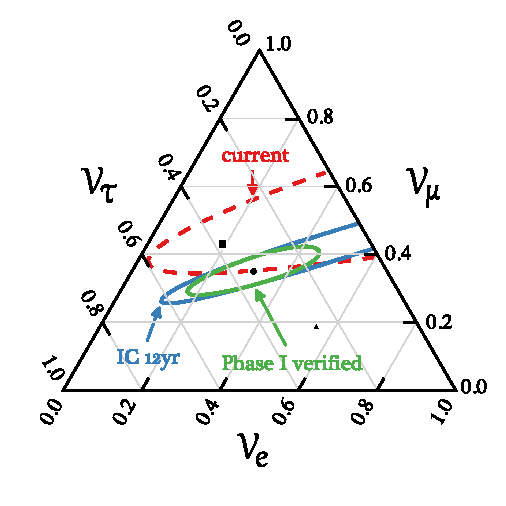
\includegraphics[scale=0.8]{\main/Cosmic/img/flavor_icecube_12years_with_taus_TickMarksB.pdf}
\vspace*{-3mm}
\caption{\label{fig:nutriangle} 
Present and future sensitivity of IceCube to the flavour composition of cosmic neutrinos. 
Each point in the triangle corresponds to a ratio
$\nu_e$  : $\nu_\mu$  : $\nu_\tau$ as measured on Earth, the individual contributions are read off the three sides of the triangle.
The red dashed contour shows the current IceCube measurement, the blue contour (label ``IC 12 yr'') shows the result expected with 12 years of the denser array DeepCore data, and the green contour (labeled ``phase I verified'') shows the result with one year of data after the deployment of 7 new strings inside DeepCore in 2022. The square, round and triangular markers show three possible results depending on the properties of the cosmic neutrino source. Any measurement outside the line connecting these three points would signal new physics in the neutrino propagation. A more precise measurement might therefore reveal the nature of the cosmic accelerator producing these neutrinos as well as non standard propagation of these particles.
}
\end{center}
\vspace*{-1cm}
\end{figure}

More than fifty years after pioneering experiments in deep underground mines in India and South Africa revealed atmospheric neutrinos, the IceCube neutrino telescope discovered a new flux for neutrino physics of extragalactic origin reaching energies over five orders of magnitude higher in energy than those of the highest energy neutrinos produced in the laboratory and ten million times those that reached us from Supernova 1987A~\cite{Ahlers:2018fkn}. The observations led to the first identification of a cosmic ray source~\cite{IceCube:2018dnn}, a rotating supermassive black hole at a distance of 4 billion lightyears. IceCube performed the first oscillation measurements over cosmic distances and found evidence for the appearance of tau neutrinos, including one event where a tau travels 17 metres through the ice before decaying. These measurements (Fig.~\ref{fig:nutriangle}) represent a powerful tool to reveal BSM neutrino physics that can be performed independently of the properties of this UHE neutrino source. IceCube identified a first Glashow-resonance event where an intermediate boson is produced in the interaction of a 6300-TeV antielectron neutrino with an atomic electron. KM3NeT-ARCA will consist of two building blocks, sparsely configured to make a very large volume detector for neutrinos of TeV to PeV energy of astrophysical origin. KM3NeT-ARCA will provide superior pointing resolution, which will enable the discovery of the neutrino sources, and a field of view including the Galactic plane.

These facilities provide unique opportunities include precision tests of fundamental symmetries, most prominently Lorentz invariance, and the search for new physics covering proton decay, dark matter trapped in the Sun, sterile neutrinos, magnetic monopoles and, in general, any hints of deviations from Standard Model physics using a neutrino beam in a new energy regime. The operating experiments have clearly demonstrated the potential of using neutrino ``telescopes" for exploring the physics of neutrinos themselves. Finally, the next Galactic supernova explosion will not only be the astronomical event of the century, it will also provide an extraordinary opportunity to do neutrino physics, as was the case with 1987A.


